\subsection{Absorpiton und Emission von elektromagnetischer Strahlung}
	Beispiel: Wasserstoffatom
		\begin{align*}
		e^- &: \text{Ladung~} q \\
		m &: \text{Masse}
		\end{align*}
		\begin{align*}
			H &= \frac{1}{2m} \left( \vec{p} + \frac{e}{c} \vec{A}' (\vec{r} , t)\right)^2
			- e \phi' (\vec{r} , t) 
			&\text{mit~} \vec{A}' &= \vec{A}_{\text{Proton}} + \underbrace{\vec{A} (\vec{r} , t)}_{\mathclap{\text{Photen von Welle}}}		
		\end{align*}
	$\vec{A}' (\vec{r} , t)$ und $\phi' (\vec{r} , t)$ sind Beiträge von elektromagnetischer Welle und vom Proton (statisch). \marginpar{das kann so auch nicht stimmen}
		\begin{align*}
			\phi' (\vec{r} , t) &= \underbrace{\frac{e}{4 \pi \hbar c}}_{\mathclap{\text{statisches Feld von Protonen}}}
			\frac{1}{r} + \phi (\vec{r} , t) \\
			H &= \underbrace{H^0}_{\mathclap{\text{ungestört von Wasserstoff-Atom (zeitunabh.)}}}
			+ \frac{e}{2 m c} \left( \vec{p} \vec{A} (\vec{r} , t) + \vec{A} (\vec{r} , t) \vec{p} + \frac{1 \cdot e^2}{2 m c^2} \vec{A}^2 (\vec{r} , t) - e\phi (\vec{r} , t) + \cdots 
			\right)
		\end{align*} 
	$e \vec{A}$ klein $\Rightarrow e^2 \vec{A}^2$ vernachlässigen \\
	$\Rightarrow$ Coulombeichung:
		\begin{itemize}
			\item $\vec{\nabla} \vec{A} = 0 \rightarrow \vec{p} \vec{A} = 0$ 
			\item $\phi (\vec{r}, t) = \text{const.} = 0$
		\end{itemize}
		\begin{equation*}
			\rightarrow H = H^0 +
			\underbrace{\frac{e}{2 m c} \vec{A} (\vec{r} , t) \vec{p}}_{\mathclap{\text{Störterm~} H^1(t)}} 
			= H^0 + H^1(t)
		\end{equation*}
	Man kann zeigen 
		\begin{equation*}
			\erw{\frac{\vec{p}}{m}} = \erw{\frac{i}{\hbar} \left[H^0 , \vec{r}\right]}
		\end{equation*}
	Nebenbedingung: Für Atome mit mehr als 1 $e^-$
		\begin{align*}
			\vec{p} &= \sum_i \vec{p}_i 
			&\rightarrow \erw{\frac{\vec{p}}{m}} &= \frac{i}{\hbar} \erw{\left[H^0 , \vec{R}\right]}
			&\text{mit~} \vec{R} &= \sum_i \vec{r}_i
		\end{align*}
	Betrachte elektromagnetische Welle
		\begin{align*}
			\vec{A}(\vec{r} , t) &= 
			\mathrm{Re} \left[ \vphantom{ \vec{A}_0 \vec{\epsilon} ~ e^{i(\vec{k} \vec{r} - \omega t)}} \right.
			\underbrace{\vec{A}_0}_{\mathclap{\in \mathds{C}}}
			~ \underbrace{\vec{\epsilon}}_{\substack{\mathds{R}^3 \text{-Polarisations-} \\ \text{vektor mit~} |\vec{\epsilon}| = 1}}
			~ e^{i(\vec{k} \vec{r} - \omega t)}
			\left. \vphantom{ \vec{A}_0 \vec{\epsilon} ~ e^{i(\vec{k} \vec{r} - \omega t)}} \right] \\
			\vec{\epsilon} ~\vec{k} &= 0
		\end{align*}
	Dispersionsrelation: 
		\begin{equation*}
			\omega = |\vec{k}| c
		\end{equation*}
	Hinweis 
		\begin{align*}
			\partial_{t} &= \vec{E} \\
			\mathrm{rot} \vec{A} &= \vec{B}
		\end{align*}
	Intensität ists bestimmt durch $A_0^2$
		\begin{align*}
			\rightarrow I &= \overline{|\vec{S}|} & \text{zeitliches Mittel ist nötig da $\vec{S}$ fluktuiert!}
		\end{align*}
	$| \vec{S} |$ ist Pointing-Vektor 
		\begin{align*}
			| \vec{S} | &= c |\vec{E}| |\vec{B}| = c |E|^2 &\text{da~} |\vec{E}| &= |\vec{B}| \text{~ in Coulombeichung} \\
			\text{mit~} \vec{E} &= \frac{1}{c} \partial_t \vec{A} 
			&\rightarrow |\vec{S}| &= \frac{1}{c} \left|\partial_t \vec{A}\right|^2
		\end{align*}
	Somit ist die Intensität:
		\begin{align*}
			I &= \underbrace{\frac{\omega}{2 c}}_{\mathclap{\text{aus zeitlichem Mittel~} \int_{0}^{2 \pi} \diff \phi \frac{1}{2 \pi} \sin^2 \phi = \frac{1}{2}}}
			|A_0|^2
		\end{align*}
	Mittlere Energiedichte der elektromagnetischen Welle
		\begin{align*}
			u (\vec{r}) &=
			\frac{1}{2} \overline{\left( E^2(\vec{r} , t) + B^2(\vec{r} , t) \right)} 
			= \frac{1}{c} \overline{|\vec{S}|} = 
			\frac{I}{c} = \frac{\omega^2}{2 c^2} |A_0|^2 \\
			\overline{u} (\omega) &= \frac{\omega^2}{2 c^2} |A_0|^2
		\end{align*}
	Störoperator in Coulombeichung
		\begin{align*}
			H^1 &= \frac{e}{2 m c} \vec{A} (\vec{r} , t) \vec{p} \\
			&= \frac{e}{m c}
			\left[A_0 e^{i(\vec{k} \vec{r} - \omega t)} ~\vec{\epsilon}~\vec{p}
			+ A^*_0 e^{-i(\vec{k} \vec{r} - \omega t)} ~\vec{\epsilon}~\vec{p}
			\right] \\
			&+ \frac{e^2}{m c^2} \underbrace{|A_0|^2}_{\mathclap{\text{sehr klein~} \rightarrow \text{~wir vernachlässigen diesen}}} 
			\left(1 + \cos \left(2 (\vec{k} \vec{r} - \omega t)\right)\right) \\
			H^1 &= \underbrace{H_\omega}_{\mathclap{\frac{e}{m c} A_0 e^{i \vec{k} \vec{r}} \vec{\epsilon}~\vec{p}}} 
			e^{-i \omega t} 
			+ H_\omega^\dagger e^{i \omega t}
		\end{align*}
	Wir wollen nun $W_{m \leftarrow n}$ ausrechnen:
		\begin{align*}
			\left|\braket{m | \frac{e}{m c} A_0 e^{i \vec{k} \vec{r}} \vec{\epsilon}~\vec{p} |n}\right|^2
			= \frac{e^2}{m^2 c^2} |A_0|^2 \left| \braket{m | e^{i \vec{k} \vec{r}} \vec{\epsilon}~\vec{p} | n}\right|^2
		\end{align*}
	Übergangsrate: Absorption: $\omega_m > \omega_n$, $\omega_m = \omega_n + \omega$
		\begin{equation*}
			W_{m \leftarrow n} = 
			\frac{1}{t \hbar} \int \limits_{-\infty}^{\infty} 
			\diff E \rho_\omega (\omega) P_{nm} (t)
		\end{equation*}
	Wir machen $t$ groß $\Rightarrow$ Fermiregeln
		\begin{align*}
			\frac{2 \pi}{\hbar} \left|\braket{m | H_\omega | n}\right|^2 &\rho_\omega (\omega) \\
			&\rho_\omega (\omega) \text{~ist Dichte von Zuständen mit~} \omega = \frac{E}{\hbar} \\
			&\text{und~ }\rho_\omega (\omega)\sim \delta (\omega + \omega_{mn})
		\end{align*}
		\begin{align*}
			W_{m \leftarrow n} &= 
			\frac{4 \pi e^2}{m^2 \hbar^2 \omega_{mn}^2} u(\omega_{mn}) 
			\left|\braket{m | e^{i \vec{k} \vec{r}} (\vec{\epsilon} \cdot \vec{p}) | n}\right|^2 \\
			\erw{\hat{p}} &= \frac{i m}{\hbar} \left[H^0 , \vec{r} \right] 
		\end{align*}
		\begin{align*}
			\text{mit~}\alpha = \frac{e^2}{4 \pi \hbar c} :
			\boxed{W_{m \leftarrow n} = \frac{16 \pi^2 \alpha c}{\hbar^3 \omega_{mn}^2} 
				u (\omega_{mn}) \left|\braket{m | e^{i \vec{k} \vec{r}} \left[H^0 , \vec{r} \cdot \vec{\epsilon}\right] | n}\right|^2
			}
		\end{align*}
	Dipolnäherung: 
		\begin{equation*}
			e^{i \vec{k} \vec{r}} = 1 + 
			\underbrace{(i \vec{k} \vec{r})}_{\substack{\mathcal{O}(\alpha)}}
		\end{equation*}
	Der $\mathcal{O}(\alpha)$ Term kann vernachlässigt werden, denn:
		\begin{align*}
			\vec{k} \cdot \vec{r} 
			&\sim \frac{\omega}{c} n^2 a_B
			\sim \frac{\alpha \hbar c}{2 n^2 a_B} \frac{n^2 a_B}{\hbar c}
			\sim \frac{\alpha}{2} \\
			\alpha &\approx \frac{1}{137} \\
			n &: \text{Hauptquantenzahl} \\	
			a_B &: \text{Bohrscher Radius}		
		\end{align*}
	Jetzt wollen wir wissen was $\braket{m | \left[H^0 , \vec{r}\right] | n}$ ist
		\begin{align*}
			\vec{\epsilon} \braket{m | \left[H^0 , \vec{r}\right] | n} 
			= \hbar \overbrace{(\omega_m - \omega_n)}^{\mathclap{\omega_{mn}}} \vec{\epsilon} \braket{m | \vec{r} | n}
		\end{align*}
	Nebenbemerkung 
		\begin{align*}
			\bra{m} H^0 &= \bra{m} \hbar \omega_m \\
			-H \ket{n} &= -\hbar \omega_n \ket{n}
		\end{align*}
		\begin{empheq}[box=\boxed]{align*}
			\text{In Dipolnäherung:} \\
					W_{m \rightarrow n} &= \frac{16 \pi^2 \alpha c}{\hbar} u(\omega_{mn}) 
					\left|\braket{m | \vec{\epsilon} \cdot \vec{r} | n}\right|^2\\
					&= \frac{4 \pi}{\hbar^2} u(\omega_{mn}) 
					\left|\braket{m | \vec{\epsilon} \cdot \vec{d} | n}\right|^2\\
					&\text{mit Dipoloperator:~} \vec{d} = e \vec{r} = \sqrt{4 \pi \hbar c \alpha} \cdot \vec{r}
		\end{empheq}
		\begin{equation*}
			\braket{\vec{r} | n \ell m} = \psi_{n \ell m} (\vec{r}) 
			= \frac{u_{n \ell}(r)}{r} Y_{\ell m} (\Theta, \phi)
		\end{equation*}
	\underline{Dipolauswahlregeln:}
		\begin{align*}
			\braket{n' \ell' m' | \vec{r} | n \ell m} &\neq 0 \\
			&\Rightarrow \int \diff \Omega~Y^*_{\ell' m'}(\Omega)~\vec{r}~Y_{\ell m} (\Omega) \neq 0 \\
			\vec{r} &= \sqrt{\frac{4 \pi}{3}} r 
			\left( \vphantom{-\frac{1}{\sqrt{2}}} \right. 
				\frac{1}{\sqrt{2}} 
				\underbrace{(-Y_{1,1} + Y_{1,-1})}_{\mathclap{\sin \Theta \cos \phi}},
				\frac{1}{\sqrt{2}} \underbrace{(Y_{1,1} + Y_{1,-1})}_{\mathclap{\sin \Theta \sin \phi}},
				Y_{1,0}
			\left. \vphantom{-\frac{1}{\sqrt{2}}} \right) \\
			&= r \sum_{i,\lambda} \vec{e}_i d_{i,\lambda} Y_{1,\lambda} \\
			&\text{wobei~} i = \{x,y,z\} \text{~und~} \lambda \in \{-1,0,1\} 
		\end{align*}
		\begin{equation*}
			Y_{1,\lambda} Y_{\ell m} = c_- Y_{\ell - 1, m + \lambda}
			+ c_0 Y_{\ell, m+\lambda} + c_+ Y_{\ell + 1, m + \lambda}
		\end{equation*}
	mit $c_-,c_0, c_+$ Clebsch-Gordon Koeffizienten.
	
	Wir führen $m' = m + \lambda$ ein, weil 
		\begin{equation*}
			\int \diff \Omega ~Y^*_{\ell', m'} Y_{L, m+\lambda} = \delta_{\ell, L} \delta_{m', m+\lambda}
		\end{equation*}
		\begin{equation*}
			\Rightarrow \boxed{\Delta m = m' - m = 0, \pm 1}
		\end{equation*}
	Paritätsoperator:
		\begin{align*}
			\mathds{P} \vec{r} &= -\vec{r} & &\mathds{P} Y_{\ell m}(\Theta, \phi) = (-)^\ell Y_{\ell m}(\Theta, \phi) \\
%		\end{align*}
%		\begin{align*}
			&\int \diff \Omega~Y_{\ell' m'}(\Omega)~\vec{r}~Y_{\ell m} (\Omega) =
			& &\text{analog zu:} \\ 
			&= \int \diff \Omega ~\mathds{P} \left(~Y^*_{\ell' m'}(\Omega)
			~\vec{r}~Y_{\ell m}(\Omega)\right)& 
			&\int\limits_{-\infty}^{\infty} \diff x f(x) 
			= \int\limits_{-\infty}^{\infty} \diff x f(-x) \\
			&= \int \diff \omega (-)^{\ell'} (-1) (-)^\ell
			\left( Y_{\ell'm'}(\Omega) ~\vec{r}~ Y_{\ell m}(\Omega)\right) \\
			&= (-)^{\ell + \ell' + 1} \int \diff \Omega ~Y_{\ell' m'}(\Omega)~\vec{r}~Y_{\ell m} (\Omega)
		\end{align*}
	Integral $\neq 0 \Rightarrow 1= (-)^{\ell + \ell' + 1} \Rightarrow \ell + \ell'$ ungerade \\
	Und dies gilt nur für $\ell' = \ell, \ell+1, \ell-1$
		\begin{empheq}[box=\boxed]{align*}
			\Rightarrow
			\Delta \ell = \ell' + \ell &= \pm 1 &\text{für~} \ell &\geq 1 \\
			&= 1 &\text{für~} \ell &= 0
		\end{empheq}
	$\Delta m = 0$ tritt nur für $\braket{\ell' , m' | z | \ell, m}$ auf \marginpar{was zur Hölle ist z?}
	
	Betrachte inkohärente Überlagerung von elektromagnetischen Wellen (keine Polarisation):
		\begin{align*}
			\frac{1}{4 \pi} \int 
			\underbrace{\diff \Omega_{\vec{\epsilon}}}_{\mathclap{\text{Mittel über alle~} \vec{\epsilon}}} 
			\left|\braket{m | \vec{d} \cdot \vec{\epsilon} | n}\right|^2 
			&= \frac{1}{4 \pi} \int \diff \Omega_{\vec{\epsilon}} 
			\braket{m | \vec{d} \cdot \vec{\epsilon} | n} \braket{n | \vec{d} \cdot \vec{\epsilon} | m} \\
			&= \sum_{i,j} \braket{m | d_i | n} \braket{n | d_j | m} 
			\frac{1}{4 \pi} \int \diff \Omega_{\vec{\epsilon}} 
			\overbrace{\epsilon_i \epsilon_j}^{\mathclap{\delta_{ij}\frac{\epsilon^2}{3}}} \\
			&= \frac{4 \pi}{3} \left|\braket{m | \vec{d} | n}\right|^2
		\end{align*} 
		\begin{empheq}[box=\boxed]{align*}
			W_{m \leftarrow n} &= 
			\frac{4 \pi}{3 \hbar^2} u (\omega_{mn}) 
			\left| \braket{n | \vec{d} | m}\right|^2 
			&\text{mit~} \vec{d} &= e \vec{r} \text{~Dipolmoment}
		\end{empheq}
		\marginpar{26.10.2015} Okay, Leute. Herr Prof. Bali hat heute eine Seite Korrektur an die Tafel geschrieben, aber ich weiß nicht wo jetzt welche 2 weg oder hin muss, denn am Ende wusste er es selbst auch nicht mehr. Deshalb schreibe ich einfach das auf, was ich mitgeschreiben habe. 
		
		Korrektur ! 
		\begin{align*}
		\vec{A} (\vec{r} , t) &=
		2 \mathrm{Re} \left(
		A_0 \vec{\epsilon} e^{i (\vec{k} \vec{r} - \omega t)}
		\right) \\
		|\vec{S}| &=
		c |\vec{E}| = \frac{\omega^2}{c} 4 |A_0|^2 \\
		u &= \frac{1}{2} \overline{\left( \vec{E}^2 + \vec{B}^2 \right)} 
		= \frac{1}{c} \overline{|\vec{S}|} 
		= \frac{\omega^2}{c^2} 2 |A_0|^2 = \frac{I}{c} \\
		H^1 &= \frac{e}{mc} \left[
		A_0 e^{i (\vec{k} \vec{r} - \omega t)} \vec{\epsilon} \vec{p} 
		+ A_0^\dagger e^{-i (\vec{k} \vec{r} - \omega t)} \vec{\epsilon} \vec{p}
		\right] \\
		&+ \frac{e^2}{m c^2} 4 |A_0|^2 \left( 1 + \cos (2 (\vec{k} \vec{r} - \omega t))\right) \\
		| \braket{m | H_\omega | n} |^2 &=	
		\frac{e^2}{4\!\!\!/ m^2 c^2} |A_0|^2
		| \braket{m | e^{i \vec{k} \vec{r}} \vec{\epsilon} \vec{p} | n} |^2 
		= \frac{e^2 u(\omega)}{2 m^2 \omega^2} 
		| \braket{m | e^{i \vec{k} \vec{r}} \vec{\epsilon} \vec{p} | n} |^2 \\
		W_{m \leftarrow n} &= \frac{4\!\!\!/ \pi e^2 u(\omega_{mn})}{m^2 \hbar^2 \omega_{mn}^2}
		|\braket{\ldots}|^2
		\end{align*}
		\begin{empheq}[box=\boxed]{align*}
		W_{m \leftarrow n} &=
		\frac{4 \pi^2 \alpha c}{\hbar^3 \omega_{mn}} u(\omega_{mn}) 
		| \braket{m | e^{i \vec{k} \vec{r}} \left[ H^0, \vec{r} \cdot \vec{\epsilon} \right]} |^2
		\end{empheq}
		Dipolnäherung:
		\begin{align*}
		W_{m \leftarrow n} &=
		\frac{4 \pi^2 \alpha c}{\hbar} u(\omega_{mn}) 
		| \braket{m | \vec{\epsilon} \cdot \vec{r} | n} |^2 
		= \frac{\pi}{\hbar^2} u(\omega_{mn}) 
		| \braket{m | \vec{\epsilon} \cdot \vec{d} | n} |^2
		\end{align*}
		\begin{align*}
		\int \diff \Omega_\epsilon \epsilon_i \epsilon_j &= c \delta_{ij} \\
		\text{Beispiel: ~} \epsilon_z &= \cos \Theta \\
		\int \diff \Omega_\epsilon \epsilon_z^2 &= 
		\int_{0}^{2 \pi} \diff \phi \int_{-1}^{1} \diff (\cos \Theta) \cos^2 \Theta 
		= 2 \pi \left. \frac{\cos^3 \Theta}{3} \right|_{-1}^1 = \frac{4 \pi}{3} \\
		\Rightarrow c &= \frac{4 \pi}{3} 
		\end{align*}
		\begin{empheq}[box=\boxed]{align*}
		W_{m \leftarrow n} = \frac{\pi}{3 \hbar^2} u(\omega_{mn})
		| \braket{n | \vec{d} | m} |^2
		\end{empheq}
		\begin{figure*} [h]
			\begin{center}
				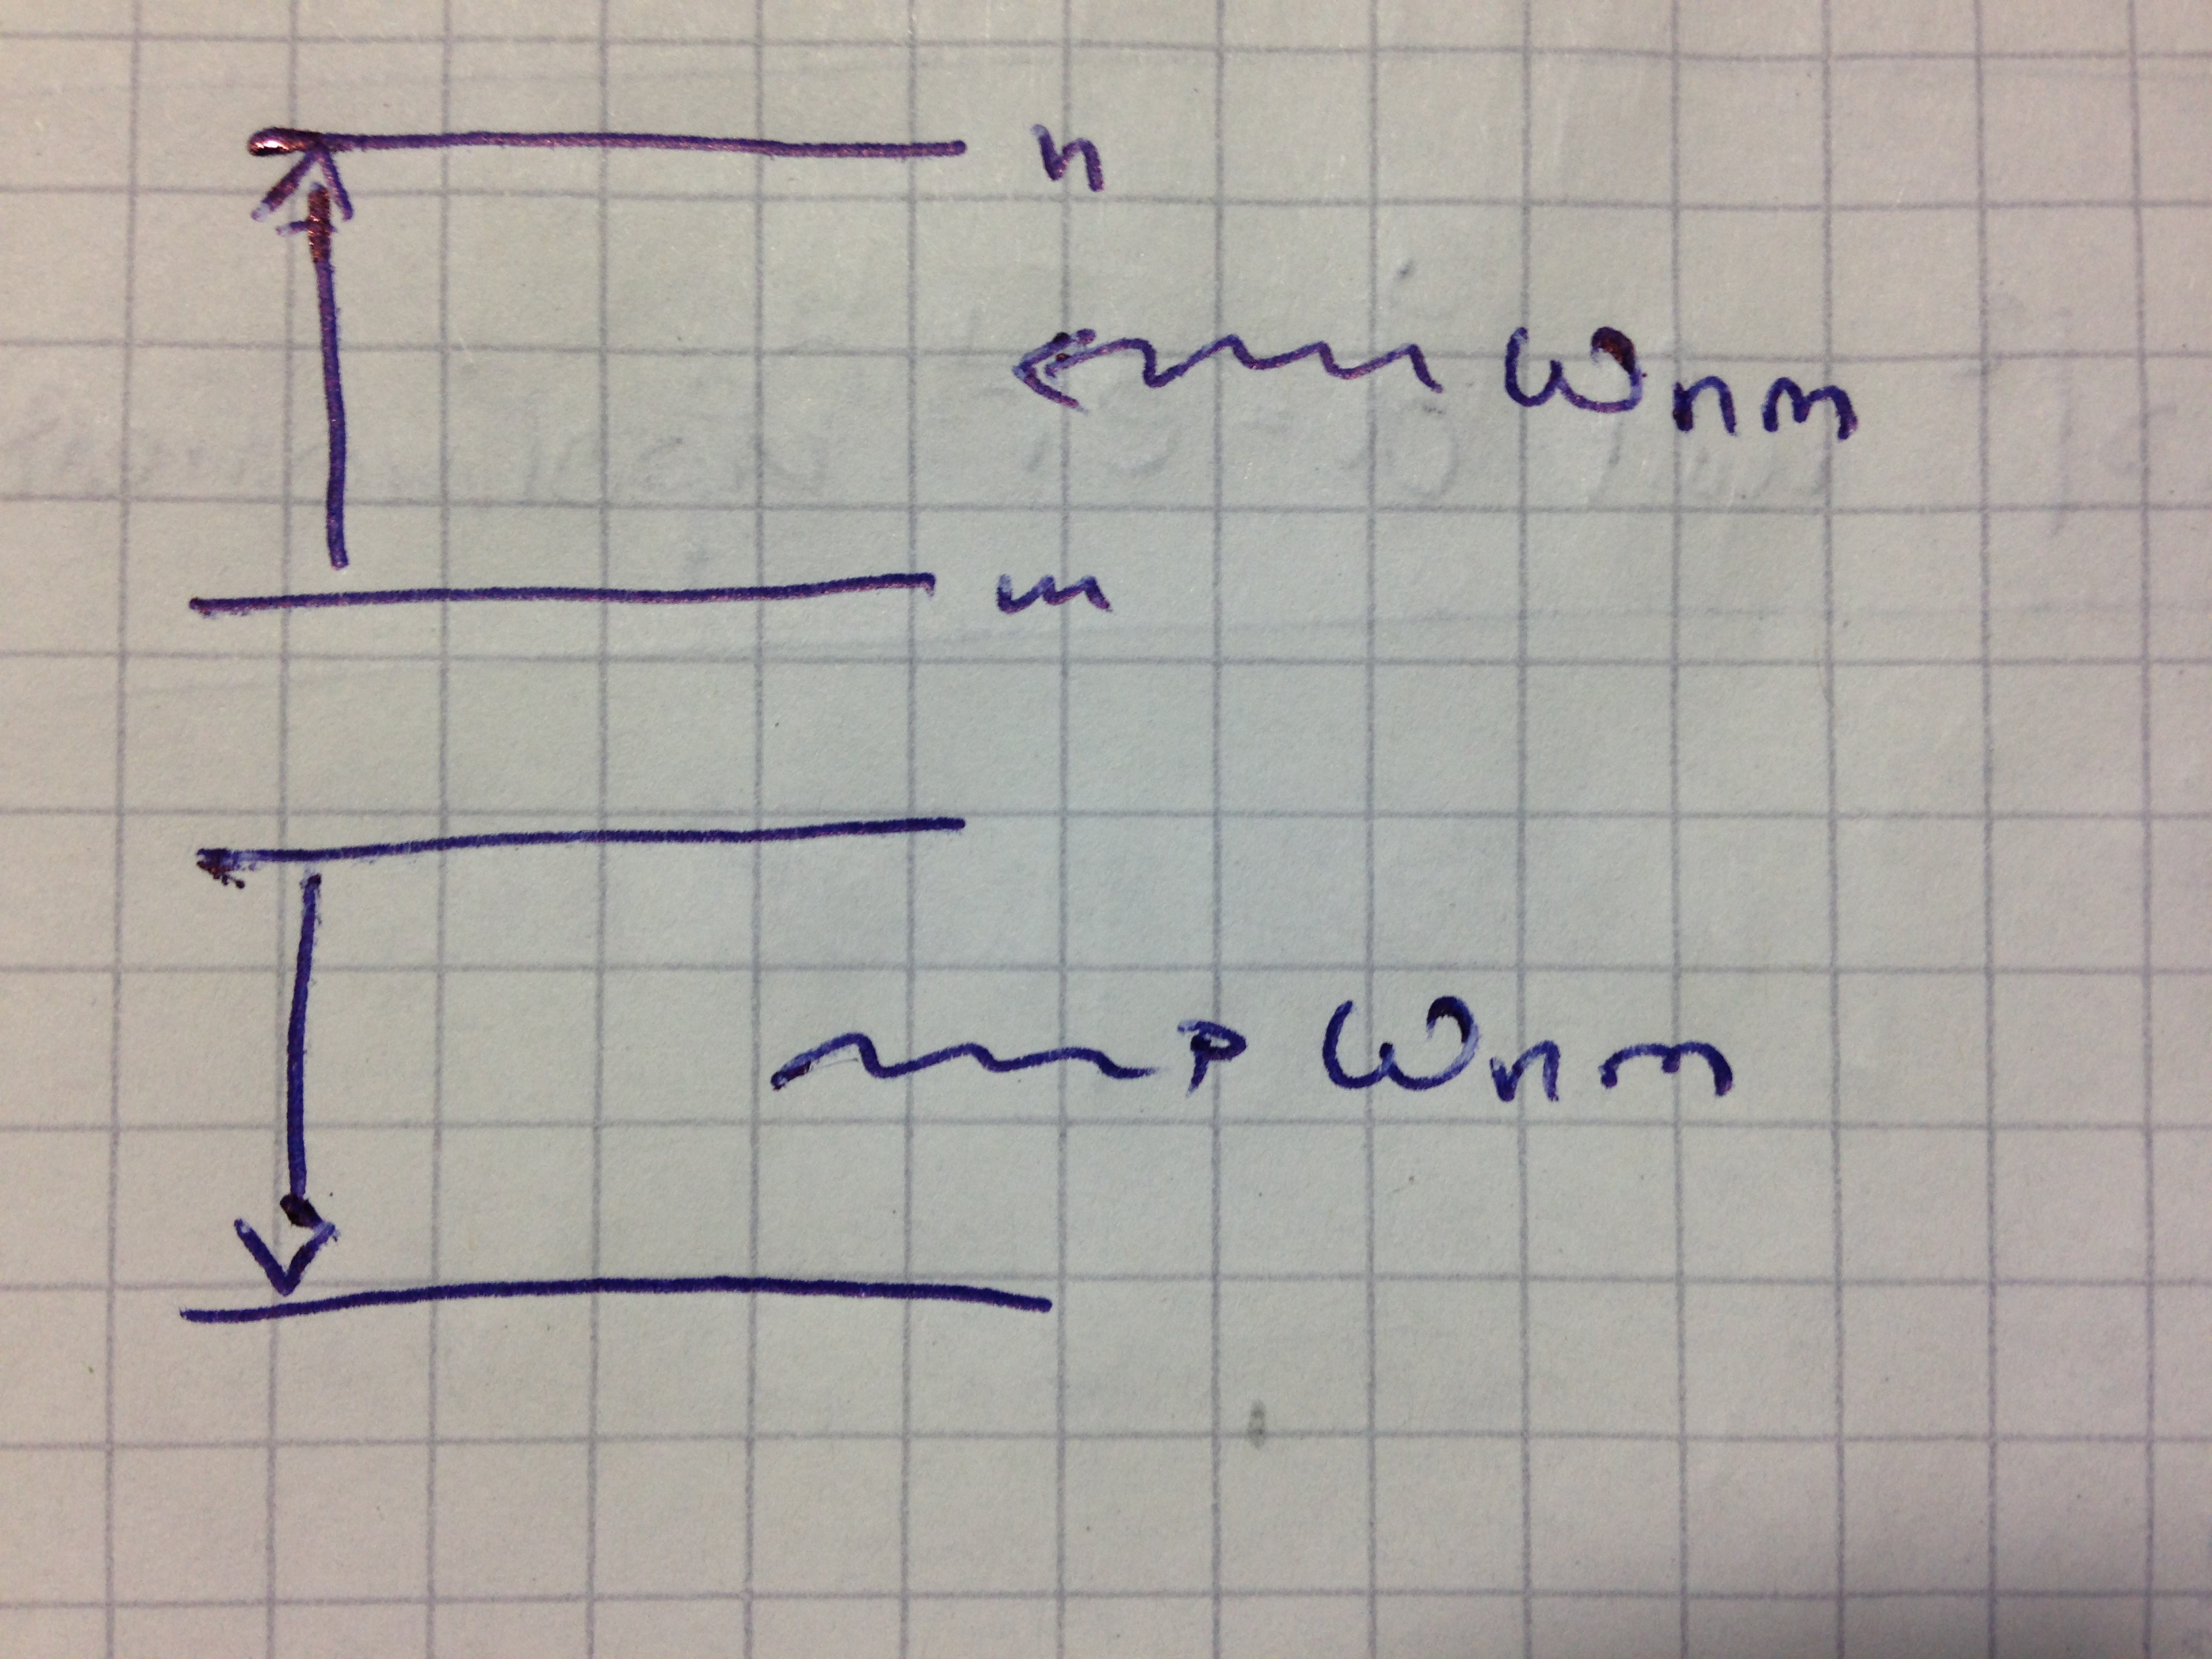
\includegraphics[width=10cm]{Bild1.jpg}
			\end{center}
		\end{figure*}
		\FloatBarrier